\subsection{Round seven results}

\label{sec:r7-results}

The corpus has 980 completed analytical-placement VPR runs (0 failed) in 1.73~h of VPR time and 450 runs of the \code{.net} arms (0 failed) in 0.82~h; Table~\ref{tab:r7corpus} lists the designs. Table~\ref{tab:r7gap} and Figure~\ref{fig:r7gap} give the hindsight gap of the \code{.net} arm, Table~\ref{tab:r7gapaff} the affinity-bias arm, Tables~\ref{tab:r7calib} and~\ref{tab:r7calibB} the calibration against the known optimum, Table~\ref{tab:r7dup} the duplication counts, and Tables~\ref{tab:r7xi} to~\ref{tab:r7coef} with Figures~\ref{fig:r7classes} and~\ref{fig:r7dist} the first mining. All mining is exploratory.

\begin{table}[t]
\caption{Round 7 corpus: logic CLBs of the stock seed-1 run, analytical-placement VPR runs completed and failed, affinity-bias rounds run, and the fixed-point arm of the affinity-bias and of the \code{.net} procedure.}
\label{tab:r7corpus}
\centering\scriptsize
\begin{tabular}{@{}lrrrrll@{}}
\toprule
design & CLBs & ok & failed & rounds & affinity arm & \code{.net} arm \\
\midrule
ch\_intrinsics & 13 & 20 & 0 & 1 & stock & net\_h2 \\
stereovision3 & 15 & 50 & 0 & 4 & h3 & net\_h3 \\
diffeq2 & 22 & 30 & 0 & 2 & h2 & net0 \\
diffeq1 & 37 & 20 & 0 & 1 & stock & net\_h1 \\
mkPktMerge & 21 & 40 & 0 & 3 & h2 & net\_h1 \\
raygentop & 143 & 20 & 0 & 1 & stock & net0 \\
sha & 142 & 20 & 0 & 1 & stock & net\_h1 \\
boundtop & 54 & 20 & 0 & 1 & stock & net0 \\
mkSMAdapter4B & 125 & 20 & 0 & 1 & stock & net\_h1 \\
or1200 & 252 & 20 & 0 & 1 & stock & net0 \\
stereovision0 & 707 & 30 & 0 & 2 & h1 & net0 \\
stereovision1 & 788 & 20 & 0 & 1 & h1 & net\_h1 \\
mkDelayWorker32B & 74 & 30 & 0 & 2 & h1 & net0 \\
stereovision2 & 1956 & 20 & 0 & 1 & stock & net0 \\
blob\_merge & 494 & 20 & 0 & 1 & stock & net\_h1 \\
n5\_mesh\_dp\_16 & 18 & 40 & 0 & 2 & h1 & net0 \\
n5\_mesh\_ctl\_16 & 18 & 50 & 0 & 3 & h2 & net\_h1 \\
n5\_tree\_dp\_16 & 18 & 40 & 0 & 2 & h1 & net\_h1 \\
n5\_tree\_ctl\_16 & 18 & 60 & 0 & 4 & h3 & net\_h2 \\
n5\_mesh\_dp\_64 & 74 & 70 & 0 & 5 & h4 & net0 \\
n5\_mesh\_ctl\_64 & 75 & 50 & 0 & 3 & h2 & net\_h1 \\
n5\_tree\_dp\_64 & 76 & 70 & 0 & 5 & h5 & net\_h1 \\
n5\_tree\_ctl\_64 & 73 & 70 & 0 & 5 & h4 & net\_h2 \\
n5\_mesh\_dp\_256 & 294 & 40 & 0 & 2 & h1 & net0 \\
n5\_mesh\_ctl\_256 & 289 & 30 & 0 & 1 & h1 & net0 \\
n5\_tree\_dp\_256 & 299 & 40 & 0 & 2 & h1 & net\_h1 \\
n5\_tree\_ctl\_256 & 296 & 40 & 0 & 2 & h1 & net\_h2 \\
\bottomrule
\end{tabular}
\end{table}

\begin{table*}[t]
\caption{Round 7, the hindsight gap of the \code{.net} arm: \code{net0} (the stock clustering, same placer) over the arm with the best median objective, in sample (geometric mean over five seeds, 95\% bootstrap interval over those seeds; above 1 means the stock clustering is worse). Fidelity is 1.0 by construction in 375 of 375 runs. Stock packing is the same in every seed, so the CLB interval has no clustering variance. Where no arm beat \code{net0} the row says so and no gap enters the median; the median is over the designs with a gain only, which is selected on the seeds it is evaluated on (winner's-curse risk). Best-known, not optimal.}
\label{tab:r7gap}
\centering\scriptsize
\begin{tabular}{@{}llllll@{}}
\toprule
design & arm & WL & CPD & CLB & W \\
\midrule
ch\_intrinsics & net\_h2 & 1.011 [0.959, 1.066] & 1.003 [0.897, 1.066] & 1.083 [1.083, 1.083] & 0.974 \\
stereovision3 & net\_h3 & 1.119 [1.065, 1.176] & 1.111 [1.028, 1.210] & 1.000 [1.000, 1.000] & 1.040 \\
diffeq2 & net0 & \multicolumn{4}{l}{no gain found (WL gap of the rounds: h1 0.921)} \\
diffeq1 & net\_h1 & 1.086 [1.054, 1.118] & 1.048 [1.008, 1.113] & 1.088 [1.088, 1.088] & 0.874 \\
mkPktMerge & net\_h1 & 1.060 [1.039, 1.080] & 1.084 [1.038, 1.131] & 1.105 [1.105, 1.105] & 0.826 \\
raygentop & net0 & \multicolumn{4}{l}{no gain found (WL gap of the rounds: h1 0.971)} \\
sha & net\_h1 & 1.038 [1.024, 1.049] & 1.033 [1.025, 1.041] & 1.000 [1.000, 1.000] & 0.950 \\
boundtop & net0 & \multicolumn{4}{l}{no gain found (WL gap of the rounds: h1 1.000)} \\
mkSMAdapter4B & net\_h1 & 0.991 [0.954, 1.023] & 0.998 [0.980, 1.017] & 1.000 [1.000, 1.000] & 0.939 \\
or1200 & net0 & \multicolumn{4}{l}{no gain found (WL gap of the rounds: h1 0.966)} \\
stereovision0 & net0 & \multicolumn{4}{l}{no gain found (WL gap of the rounds: h1 0.952)} \\
stereovision1 & net\_h1 & 0.986 [0.972, 0.999] & 1.058 [1.005, 1.129] & 1.033 [1.033, 1.033] & 0.868 \\
mkDelayWorker32B & net0 & \multicolumn{4}{l}{no gain found (WL gap of the rounds: h1 0.974)} \\
stereovision2 & net0 & \multicolumn{4}{l}{no gain found (WL gap of the rounds: h1 0.976)} \\
blob\_merge & net\_h1 & 1.041 [1.015, 1.070] & 0.981 [0.962, 1.000] & 1.019 [1.019, 1.019] & 0.895 \\
\midrule
median over the 8 designs with a gain & & 1.040 & 1.041 & 1.026 & 0.917 \\
\bottomrule
\end{tabular}
\end{table*}

\begin{figure}[t]
\centering
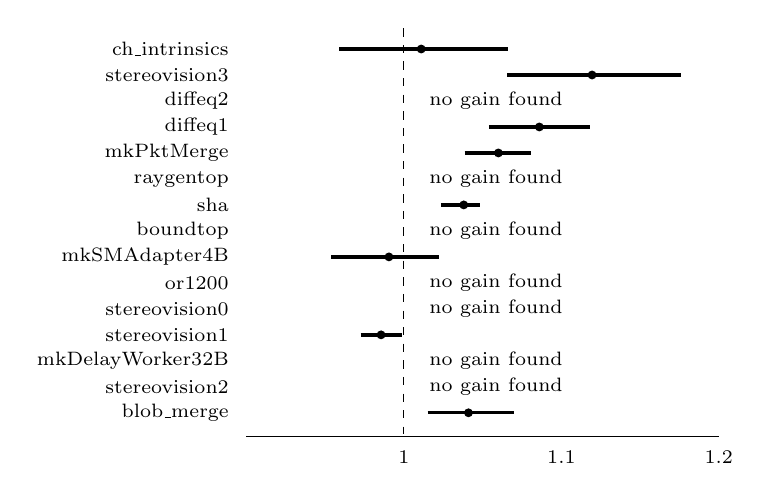
\begin{tikzpicture}[x=1cm,y=0.33cm,font=\scriptsize]
\node[anchor=east] at (-0.1,0) {ch\_intrinsics};
\draw[line width=1.2pt] (1.18,0) -- (3.32,0);
\fill (2.22,0) circle (1.6pt);
\node[anchor=east] at (-0.1,-1) {stereovision3};
\draw[line width=1.2pt] (3.31,-1) -- (5.52,-1);
\fill (4.39,-1) circle (1.6pt);
\node[anchor=east] at (-0.1,-2) {diffeq2};
\node[anchor=west] at (2.20,-2) {no gain found};
\node[anchor=east] at (-0.1,-3) {diffeq1};
\draw[line width=1.2pt] (3.08,-3) -- (4.36,-3);
\fill (3.72,-3) circle (1.6pt);
\node[anchor=east] at (-0.1,-4) {mkPktMerge};
\draw[line width=1.2pt] (2.77,-4) -- (3.61,-4);
\fill (3.20,-4) circle (1.6pt);
\node[anchor=east] at (-0.1,-5) {raygentop};
\node[anchor=west] at (2.20,-5) {no gain found};
\node[anchor=east] at (-0.1,-6) {sha};
\draw[line width=1.2pt] (2.47,-6) -- (2.97,-6);
\fill (2.76,-6) circle (1.6pt);
\node[anchor=east] at (-0.1,-7) {boundtop};
\node[anchor=west] at (2.20,-7) {no gain found};
\node[anchor=east] at (-0.1,-8) {mkSMAdapter4B};
\draw[line width=1.2pt] (1.08,-8) -- (2.45,-8);
\fill (1.81,-8) circle (1.6pt);
\node[anchor=east] at (-0.1,-9) {or1200};
\node[anchor=west] at (2.20,-9) {no gain found};
\node[anchor=east] at (-0.1,-10) {stereovision0};
\node[anchor=west] at (2.20,-10) {no gain found};
\node[anchor=east] at (-0.1,-11) {stereovision1};
\draw[line width=1.2pt] (1.45,-11) -- (1.98,-11);
\fill (1.71,-11) circle (1.6pt);
\node[anchor=east] at (-0.1,-12) {mkDelayWorker32B};
\node[anchor=west] at (2.20,-12) {no gain found};
\node[anchor=east] at (-0.1,-13) {stereovision2};
\node[anchor=west] at (2.20,-13) {no gain found};
\node[anchor=east] at (-0.1,-14) {blob\_merge};
\draw[line width=1.2pt] (2.30,-14) -- (3.40,-14);
\fill (2.82,-14) circle (1.6pt);
\draw[dashed] (2.00,0.8) -- (2.00,-14.8);
\draw (0,-14.9) -- (6,-14.9);
\node at (2.00,-15.7) {1};
\node at (4.00,-15.7) {1.1};
\node at (6.00,-15.7) {1.2};
\end{tikzpicture}
\caption{Round 7: wirelength gap net0$/$hindsight per design for the \code{.net} arm (dot: geometric mean over the five seeds, in sample, bar: 95\% bootstrap interval over those seeds). Designs where the procedure found no gain carry no dot. Above 1, the stock clustering routes longer wires than the best-known one.}
\label{fig:r7gap}
\end{figure}

\begin{table*}[t]
\caption{Round 7, the affinity-bias arm (the Norns packer with an affinity file at weight 100, analytical-placement flow, stock over arm, geometric mean over ten seeds with 95\% bootstrap interval; the arm and its source run were chosen on the same seeds, so the gap is optimistic by selection; the out-of-sample check is in the text). This is the gap reachable via affinity bias, not a lower bound on the gap between the packer and a best-known clustering: the packer rebuilds only part of the requested groups (fidelity: share of the groups built whole). A design whose fidelity stays below 0.5 in every round is marked ``not realised'' (protocol stop rule) and left out of the median; where no arm beat stock the row says so and no gap enters the median.}
\label{tab:r7gapaff}
\centering\scriptsize
\begin{tabular}{@{}llllllr@{}}
\toprule
design & arm & WL & CPD & CLB & W & fidelity \\
\midrule
ch\_intrinsics & stock & \multicolumn{4}{l}{no gain found (WL gap of the rounds: h1 0.987)} & 0.58 \\
stereovision3 & h3 & 1.098 [1.048, 1.148] & 1.050 [0.988, 1.119] & 1.000 [1.000, 1.000] & 0.958 & 0.47 (not realised) \\
diffeq2 & h2 & 0.997 [0.928, 1.061] & 1.011 [0.952, 1.061] & 1.000 [1.000, 1.000] & 0.994 & 0.79 \\
diffeq1 & stock & \multicolumn{4}{l}{no gain found (WL gap of the rounds: h1 0.959)} & 0.45 (not realised) \\
mkPktMerge & h2 & 1.024 [0.989, 1.059] & 1.033 [1.011, 1.054] & 1.000 [1.000, 1.000] & 0.988 & 0.56 \\
raygentop & stock & \multicolumn{4}{l}{no gain found (WL gap of the rounds: h1 0.965)} & 0.40 (not realised) \\
sha & stock & \multicolumn{4}{l}{no gain found (WL gap of the rounds: h1 0.970)} & 0.60 \\
boundtop & stock & \multicolumn{4}{l}{no gain found (WL gap of the rounds: h1 1.025)} & 0.58 \\
mkSMAdapter4B & stock & \multicolumn{4}{l}{no gain found (WL gap of the rounds: h1 0.985)} & 0.39 (not realised) \\
or1200 & stock & \multicolumn{4}{l}{no gain found (WL gap of the rounds: h1 0.985)} & 0.32 (not realised) \\
stereovision0 & h1 & 0.985 [0.959, 1.015] & 1.038 [0.980, 1.114] & 1.017 [1.017, 1.017] & 0.971 & 0.75 \\
stereovision1 & h1 & 0.985 [0.975, 0.995] & 1.005 [0.925, 1.090] & 1.006 [1.006, 1.006] & 0.994 & 0.50 (not realised) \\
mkDelayWorker32B & h1 & 1.009 [0.998, 1.021] & 1.003 [0.992, 1.014] & 1.057 [1.057, 1.057] & 1.000 & 0.49 (not realised) \\
stereovision2 & stock & \multicolumn{4}{l}{no gain found (WL gap of the rounds: h1 0.997)} & 0.78 \\
blob\_merge & stock & \multicolumn{4}{l}{no gain found (WL gap of the rounds: h1 0.981)} & 0.71 \\
\midrule
median over the 3 designs with a gain and fidelity $\ge$ 0.5 & & 0.997 & 1.033 & 1.000 & 0.988 & 0.75 \\
\bottomrule
\end{tabular}
\end{table*}

\begin{table*}[t]
\caption{Round 7, calibration on the round-5 constructions, \code{.net} arm (in sample): \code{net0} over the known clustering (known) and over the hindsight arm (H) for wirelength and CLB count, and the recovery $(\ln \mathrm{net0}-\ln H)/(\ln \mathrm{net0}-\ln \mathrm{known})$ from the geometric means over the seeds (``none'': the known clustering is less than 5\% better, nothing to recover). The last column is the recovery of the critical-path delay.}
\label{tab:r7calib}
\centering\scriptsize
\begin{tabular}{@{}lrrrrrrr@{}}
\toprule
design & WL known & WL H & WL rec. & CLB known & CLB H & CLB rec. & CPD rec. \\
\midrule
n5\_mesh\_dp\_16 & 1.476 & no gain & none & 1.125 & no gain & none & none \\
n5\_mesh\_ctl\_16 & 1.457 & 1.068 & 0.18 & 1.125 & 1.000 & 0.00 & -0.05 \\
n5\_tree\_dp\_16 & 1.200 & 1.222 & 1.10 & 1.125 & 1.125 & 1.00 & none \\
n5\_tree\_ctl\_16 & 1.953 & 1.688 & 0.78 & 1.125 & 1.059 & 0.49 & 1.21 \\
n5\_mesh\_dp\_64 & 1.495 & no gain & none & 1.156 & no gain & none & none \\
n5\_mesh\_ctl\_64 & 1.494 & 1.149 & 0.35 & 1.172 & 1.042 & 0.26 & 1.39 \\
n5\_tree\_dp\_64 & 1.908 & 1.305 & 0.41 & 1.188 & 1.070 & 0.40 & 0.79 \\
n5\_tree\_ctl\_64 & 1.798 & 1.090 & 0.15 & 1.141 & 1.028 & 0.21 & 0.70 \\
n5\_mesh\_dp\_256 & 1.198 & no gain & none & 1.148 & no gain & none & none \\
n5\_mesh\_ctl\_256 & 1.333 & no gain & none & 1.129 & no gain & none & none \\
n5\_tree\_dp\_256 & 1.751 & 1.165 & 0.27 & 1.168 & 1.057 & 0.35 & 0.31 \\
n5\_tree\_ctl\_256 & 1.560 & 1.170 & 0.35 & 1.156 & 1.072 & 0.48 & 0.32 \\
\bottomrule
\end{tabular}
\end{table*}

\begin{table}[t]
\caption{Round 7, recovery of the known-clustering gap, median over the designs of a size where the known clustering is at least 5\% better, by block count $B$ (designs with a recovery defined / designs of that size). Recovery is computed from the aggregated geometric means over seeds. A median of 1 would mean the procedure reaches the known clustering.}
\label{tab:r7calibB}
\centering\scriptsize
\begin{tabular}{@{}llrrr@{}}
\toprule
arm & $B$ & WL & CLB & CPD \\
\midrule
\code{.net} & $B$=16 & 0.78 (3/4) & 0.49 (3/4) & 0.58 (2/4) \\
\code{.net} & $B$=64 & 0.35 (3/4) & 0.26 (3/4) & 0.79 (3/4) \\
\code{.net} & $B$=256 & 0.31 (2/4) & 0.42 (2/4) & 0.31 (2/4) \\
\code{.net} & all & 0.35 (8/12) & 0.38 (8/12) & 0.70 (7/12) \\
affinity-bias & $B$=16 & 1.00 (4/4) & 1.00 (4/4) & 1.00 (3/4) \\
affinity-bias & $B$=64 & 0.42 (4/4) & 0.78 (4/4) & 0.77 (4/4) \\
affinity-bias & $B$=256 & 0.19 (4/4) & 0.56 (4/4) & 0.29 (4/4) \\
affinity-bias & all & 0.52 (12/12) & 0.70 (12/12) & 0.72 (11/12) \\
\bottomrule
\end{tabular}
\end{table}

\begin{table}[t]
\caption{Round 7, LUT duplication candidates (single-LUT drivers with sinks in two or more logic CLBs; pad and hard-block sinks do not count), median over the ten stock seeds of per-run values: count, share of all LUTs, share within 5\% and 10\% of the critical-path delay (a lower bound: criticality comes from the 200 reported paths, so a candidate on an unreported path counts as not critical), and the upper estimate of the delay saved if every candidate hop were free (share of CPD; stock, then the affinity-bias arm where it found a gain, `--' otherwise). Last column: LUTs that count only through one logic CLB plus a pad or hard block. Nothing is built.}
\label{tab:r7dup}
\centering\scriptsize
\begin{tabular}{@{}lrrrrrrr@{}}
\toprule
design & cand. & of LUTs & near 5\% & near 10\% & saved & saved (H) & other \\
\midrule
ch\_intrinsics & 1.00 & 1.0\% & 0.0\% & 0.0\% & 0.0\% & -- & 3.00 \\
stereovision3 & 15.00 & 8.8\% & 6.7\% & 6.7\% & 13.6\% & 14.9\% & 0.00 \\
diffeq2 & 8.00 & 4.0\% & 0.0\% & 0.0\% & 0.0\% & 0.0\% & 0.00 \\
diffeq1 & 7.00 & 2.4\% & 0.0\% & 0.0\% & 0.0\% & -- & 0.00 \\
mkPktMerge & 2.00 & 1.1\% & 0.0\% & 0.0\% & 0.0\% & 0.0\% & 1.00 \\
raygentop & 58.00 & 5.4\% & 0.0\% & 0.0\% & 0.0\% & -- & 2.00 \\
sha & 31.00 & 2.4\% & 6.5\% & 6.5\% & 9.5\% & -- & 0.00 \\
boundtop & 18.00 & 3.5\% & 11.1\% & 11.1\% & 6.6\% & -- & 13.00 \\
mkSMAdapter4B & 86.00 & 8.1\% & 2.3\% & 7.0\% & 7.7\% & -- & 4.00 \\
or1200 & 336.00 & 14.0\% & 0.0\% & 3.9\% & 0.0\% & -- & 123.00 \\
stereovision0 & 105.00 & 1.5\% & 2.9\% & 8.6\% & 12.5\% & 12.7\% & 0.00 \\
\bottomrule
\end{tabular}
\end{table}

\begin{table}[t]
\caption{Round 7 (exploratory), Table~\ref{tab:r3status} re-measured at each level of the HDL chain: the stratified distance difference $d_r$ (related minus unrelated pairs within net-connectivity strata, as a fraction of the unrelated mean; negative means closer than the nets predict), median over designs, designs with $d_r<0$, the range of the same statistic on label-shuffled data, and the share of the shuffles at or below the observed median. Levels that exist in the data are tested; a level identical to a shallower one is not tested again.}
\label{tab:r7xi}
\centering\scriptsize
\begin{tabular}{@{}lrrcr@{}}
\toprule
relation & median $d_r$ & $d_r<0$ & null range & null$\le$obs \\
\midrule
same bit index & 0.012 & 7/15 & [-0.008, 0.009] & 1.000 \\
same instance, depth 1 & -0.135 & 11/14 & [-0.006, 0.006] & 0.005 \\
same instance, depth 2 & n/a & 0/0 & [n/a, n/a] & n/a \\
same instance, depth 3 & n/a & 0/0 & [n/a, n/a] & n/a \\
same instance (full path) & \multicolumn{4}{l}{identical to same instance, depth 1: the instance chain has depth 1} \\
same statement & -0.174 & 14/15 & [-0.006, 0.006] & 0.005 \\
same word & -0.414 & 14/15 & [-0.015, 0.014] & 0.005 \\
same word and bit & -0.276 & 2/2 & [-0.418, 0.521] & 0.100 \\
\bottomrule
\end{tabular}
\end{table}

\begin{table}[t]
\caption{Round 7 (exploratory), held-out-family models, target co-location in the \code{.net} hindsight clustering, designs where it beat \code{net0}: 8 designs in 6 families (blob\_merge, ch\_intrinsics, diffeq, mk, sha, stereovision). Baseline (net connectivity, criticality, kinds, stock co-CLB and stock distance, no HDL): AUC on connected pairs mean 0.948, median 0.963; on uniform pairs mean 0.949. Change from adding HDL features: mean and median over held-out designs, bootstrap interval of the mean, designs improved, and the same change with the HDL labels (and the carry flag) shuffled, 200 shuffles.}
\label{tab:r7modelnet}
\centering\scriptsize
\begin{tabular}{@{}lrrcrc@{}}
\toprule
change & mean & median & 95\% CI & better & shuffled null \\
\midrule
AUC (connected pairs), bit features & 0.000 & 0.000 & [-0.001, 0.002] & 5/8 & 0.000 [-0.000, 0.001] \\
AUC (connected pairs), all HDL & 0.003 & 0.002 & [-0.000, 0.006] & 6/8 & -0.000 [-0.001, 0.001] \\
AUC (uniform pairs), all HDL & 0.004 & 0.003 & [0.001, 0.007] & 7/8 & -0.000 [-0.001, -0.000] \\
$R^2$ of normalised distance, bit features & 0.004 & 0.001 & [-0.000, 0.010] & 6/8 & -0.004 [-0.005, -0.003] \\
$R^2$ of normalised distance, all HDL & -0.048 & -0.047 & [-0.091, -0.008] & 1/8 & -0.055 [-0.065, -0.045] \\
\bottomrule
\end{tabular}
\end{table}

\begin{table}[t]
\caption{Round 7 (exploratory), held-out-family models, target co-location in the best affinity-bias run, designs where it beat stock: 6 designs in 3 families (diffeq, mk, stereovision). Baseline (net connectivity, criticality, kinds, stock co-CLB and stock distance, no HDL): AUC on connected pairs mean 0.944, median 0.965; on uniform pairs mean 0.965. Change from adding HDL features: mean and median over held-out designs, bootstrap interval of the mean, designs improved, and the same change with the HDL labels (and the carry flag) shuffled, 200 shuffles.}
\label{tab:r7modelaff}
\centering\scriptsize
\begin{tabular}{@{}lrrcrc@{}}
\toprule
change & mean & median & 95\% CI & better & shuffled null \\
\midrule
AUC (connected pairs), bit features & -0.001 & -0.001 & [-0.006, 0.003] & 1/6 & -0.001 [-0.002, 0.000] \\
AUC (connected pairs), all HDL & 0.006 & -0.000 & [-0.001, 0.018] & 2/6 & -0.000 [-0.001, 0.000] \\
AUC (uniform pairs), all HDL & 0.005 & 0.004 & [0.002, 0.009] & 6/6 & -0.000 [-0.000, 0.000] \\
$R^2$ of normalised distance, bit features & -0.000 & -0.001 & [-0.004, 0.005] & 3/6 & -0.007 [-0.009, -0.005] \\
$R^2$ of normalised distance, all HDL & -0.048 & -0.070 & [-0.131, 0.051] & 1/6 & -0.095 [-0.115, -0.077] \\
\bottomrule
\end{tabular}
\end{table}

\begin{table}[t]
\caption{Round 7 (exploratory), held-out-family models, target co-location in the best affinity-bias run, all designs (variant: includes designs where hindsight equals stock): 15 designs in 9 families (blob\_merge, boundtop, ch\_intrinsics, diffeq, mk, or1200, raygentop, sha, stereovision). Baseline (net connectivity, criticality, kinds, stock co-CLB and stock distance, no HDL): AUC on connected pairs mean 0.949, median 0.959; on uniform pairs mean 0.964. Change from adding HDL features: mean and median over held-out designs, bootstrap interval of the mean, designs improved, and the same change with the HDL labels (and the carry flag) shuffled, 200 shuffles.}
\label{tab:r7modelaffall}
\centering\scriptsize
\begin{tabular}{@{}lrrcrc@{}}
\toprule
change & mean & median & 95\% CI & better & shuffled null \\
\midrule
AUC (connected pairs), bit features & 0.001 & 0.001 & [-0.001, 0.003] & 10/15 & -0.000 [-0.000, 0.000] \\
AUC (connected pairs), all HDL & 0.004 & 0.002 & [0.000, 0.008] & 10/15 & -0.000 [-0.001, 0.000] \\
AUC (uniform pairs), all HDL & 0.003 & 0.002 & [0.001, 0.005] & 14/15 & -0.000 [-0.000, 0.000] \\
$R^2$ of normalised distance, bit features & -0.001 & 0.000 & [-0.004, 0.001] & 8/15 & -0.002 [-0.002, -0.002] \\
$R^2$ of normalised distance, all HDL & -0.027 & -0.022 & [-0.048, -0.006] & 2/15 & -0.044 [-0.047, -0.041] \\
\bottomrule
\end{tabular}
\end{table}

\begin{table}[t]
\caption{Round 7 (exploratory), stability across seeds. The stock clustering barely depends on the seed (100.0\% of the universe pairs have the same co-CLB status in all ten stock runs), so stability is read on placement: of the 625919 pairs of the unbiased samples within two CLBs in at least one seed, 196982 (31.5\%) are within two CLBs in eight or more of ten. Share of stable pairs given the relation and given its absence, their difference, and the label-shuffled range of the difference. By N17 class: SC 77.4\%, SN 80.2\%, SI 43.9\%, OR 30.4\%, FL 11.7\%.}
\label{tab:r7stab}
\centering\scriptsize
\begin{tabular}{@{}lrrrc@{}}
\toprule
relation & stable $|$ rel. & stable $|$ not & diff. & null range \\
\midrule
same bit index & 48.7\% & 30.9\% & 0.178 & [0.109, 0.129] \\
same instance, depth 1 & 36.1\% & 20.9\% & 0.153 & [-0.162, -0.156] \\
same instance, depth 2 & n/a & 31.5\% & n/a & [n/a, n/a] \\
same instance, depth 3 & n/a & 31.5\% & n/a & [n/a, n/a] \\
same instance (full path) & 36.1\% & 20.9\% & 0.153 & [-0.162, -0.156] \\
same statement & 47.7\% & 22.5\% & 0.252 & [-0.101, -0.092] \\
same word & 84.4\% & 27.1\% & 0.573 & [-0.036, -0.011] \\
same word and bit & n/a & 31.5\% & n/a & [-0.315, 0.685] \\
\bottomrule
\end{tabular}
\end{table}

\begin{table}[t]
\caption{Round 7 (exploratory), where stock packing and the best affinity-bias hindsight run disagree (against the stock run of the same seed; 132189 pairs joined by hindsight only, 129313 by stock only, 1116107 by both). Enrichment of each relation among the disagreement pairs over its share among the pairs of the universe (the unbiased samples; protocol baseline), with the label-shuffled range; the earlier baseline, the pairs both clusterings join, is kept in the data file as a logged deviation.}
\label{tab:r7disagree}
\centering\scriptsize
\begin{tabular}{@{}lrcrc@{}}
\toprule
relation & hindsight only & null & stock only & null \\
\midrule
same bit index & 1.54 & [1.47, 1.59] & 2.36 & [1.45, 1.58] \\
same instance, depth 1 & 1.12 & [0.56, 0.58] & 1.15 & [0.57, 0.58] \\
same instance, depth 2 & n/a & [n/a, n/a] & n/a & [n/a, n/a] \\
same instance, depth 3 & n/a & [n/a, n/a] & n/a & [n/a, n/a] \\
same instance (full path) & 1.12 & [0.56, 0.58] & 1.15 & [0.57, 0.58] \\
same statement & 2.08 & [0.67, 0.71] & 2.15 & [0.68, 0.72] \\
same word & 3.14 & [0.50, 0.58] & 3.45 & [0.50, 0.59] \\
same word and bit & 0.00 & [0.00, 7.04] & 0.00 & [0.00, 6.74] \\
\bottomrule
\end{tabular}
\end{table}

\begin{table}[t]
\caption{Round 7 (exploratory), coefficients of the features in the full logistic model for hindsight co-location in the first model variant with designs (standardised features; mean over the held-out folds with a bootstrap interval over folds). The bit-level hint question (Peter 2026-10-26) is the rows ``same bit index'', ``same word and bit'', ``bit close'' and ``carry nb''.}
\label{tab:r7coef}
\centering\scriptsize
\begin{tabular}{@{}lrc@{}}
\toprule
feature & coefficient & 95\% CI \\
\midrule
bit close & 0.005 & [-0.013, 0.024] \\
carry nb & 0.081 & [0.062, 0.108] \\
co stock & 0.207 & [0.183, 0.231] \\
kind adder & -0.130 & [-0.143, -0.115] \\
kind ff & -0.040 & [-0.059, -0.022] \\
kind lf & 0.117 & [0.108, 0.127] \\
kind ll & 0.040 & [0.025, 0.054] \\
log dist stock & -2.214 & [-2.418, -1.982] \\
log minfan & -0.490 & [-0.511, -0.470] \\
log nshared & 0.248 & [0.219, 0.276] \\
pcrit max & -0.203 & [-0.244, -0.166] \\
pcrit min & 0.241 & [0.209, 0.277] \\
same bit index & 0.023 & [0.005, 0.038] \\
same instance, depth 1 & -0.052 & [-0.060, -0.044] \\
same instance, depth 2 & 0.000 & [0.000, 0.000] \\
same instance, depth 3 & 0.000 & [0.000, 0.000] \\
same instance (full path) & -0.052 & [-0.060, -0.044] \\
same statement & 0.044 & [0.033, 0.055] \\
same word & 0.264 & [0.214, 0.309] \\
same word and bit & 0.000 & [0.000, 0.000] \\
scrit & -0.080 & [-0.105, -0.053] \\
series & 0.362 & [0.317, 0.404] \\
shared only & 0.328 & [0.296, 0.350] \\
\bottomrule
\end{tabular}
\end{table}

\begin{figure}[t]
\centering
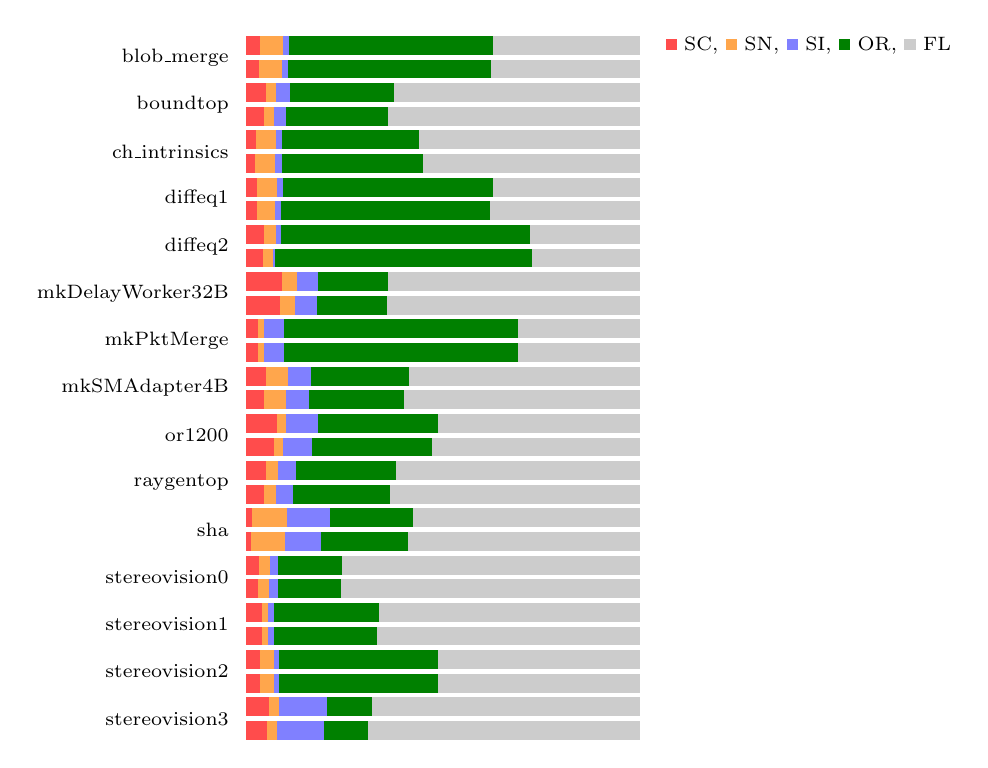
\begin{tikzpicture}[x=1cm,y=0.3cm,font=\scriptsize]
\node[anchor=east] at (-0.1,-0.5) {blob\_merge};
\fill[red!70] (0.000,-0.4) rectangle (0.167,0.4);
\fill[orange!70] (0.167,-0.4) rectangle (0.459,0.4);
\fill[blue!50] (0.459,-0.4) rectangle (0.546,0.4);
\fill[green!50!black] (0.546,-0.4) rectangle (3.127,0.4);
\fill[gray!40] (3.127,-0.4) rectangle (5.000,0.4);
\fill[red!70] (0.000,-1.4) rectangle (0.166,-0.6);
\fill[orange!70] (0.166,-1.4) rectangle (0.453,-0.6);
\fill[blue!50] (0.453,-1.4) rectangle (0.534,-0.6);
\fill[green!50!black] (0.534,-1.4) rectangle (3.112,-0.6);
\fill[gray!40] (3.112,-1.4) rectangle (5.000,-0.6);
\node[anchor=east] at (-0.1,-2.5) {boundtop};
\fill[red!70] (0.000,-2.4) rectangle (0.252,-1.6);
\fill[orange!70] (0.252,-2.4) rectangle (0.375,-1.6);
\fill[blue!50] (0.375,-2.4) rectangle (0.549,-1.6);
\fill[green!50!black] (0.549,-2.4) rectangle (1.879,-1.6);
\fill[gray!40] (1.879,-2.4) rectangle (5.000,-1.6);
\fill[red!70] (0.000,-3.4) rectangle (0.229,-2.6);
\fill[orange!70] (0.229,-3.4) rectangle (0.349,-2.6);
\fill[blue!50] (0.349,-3.4) rectangle (0.503,-2.6);
\fill[green!50!black] (0.503,-3.4) rectangle (1.800,-2.6);
\fill[gray!40] (1.800,-3.4) rectangle (5.000,-2.6);
\node[anchor=east] at (-0.1,-4.5) {ch\_intrinsics};
\fill[red!70] (0.000,-4.4) rectangle (0.126,-3.6);
\fill[orange!70] (0.126,-4.4) rectangle (0.373,-3.6);
\fill[blue!50] (0.373,-4.4) rectangle (0.455,-3.6);
\fill[green!50!black] (0.455,-4.4) rectangle (2.196,-3.6);
\fill[gray!40] (2.196,-4.4) rectangle (5.000,-3.6);
\fill[red!70] (0.000,-5.4) rectangle (0.111,-4.6);
\fill[orange!70] (0.111,-5.4) rectangle (0.365,-4.6);
\fill[blue!50] (0.365,-5.4) rectangle (0.450,-4.6);
\fill[green!50!black] (0.450,-5.4) rectangle (2.242,-4.6);
\fill[gray!40] (2.242,-5.4) rectangle (5.000,-4.6);
\node[anchor=east] at (-0.1,-6.5) {diffeq1};
\fill[red!70] (0.000,-6.4) rectangle (0.138,-5.6);
\fill[orange!70] (0.138,-6.4) rectangle (0.383,-5.6);
\fill[blue!50] (0.383,-6.4) rectangle (0.464,-5.6);
\fill[green!50!black] (0.464,-6.4) rectangle (3.129,-5.6);
\fill[gray!40] (3.129,-6.4) rectangle (5.000,-5.6);
\fill[red!70] (0.000,-7.4) rectangle (0.137,-6.6);
\fill[orange!70] (0.137,-7.4) rectangle (0.367,-6.6);
\fill[blue!50] (0.367,-7.4) rectangle (0.440,-6.6);
\fill[green!50!black] (0.440,-7.4) rectangle (3.088,-6.6);
\fill[gray!40] (3.088,-7.4) rectangle (5.000,-6.6);
\node[anchor=east] at (-0.1,-8.5) {diffeq2};
\fill[red!70] (0.000,-8.4) rectangle (0.217,-7.6);
\fill[orange!70] (0.217,-8.4) rectangle (0.376,-7.6);
\fill[blue!50] (0.376,-8.4) rectangle (0.433,-7.6);
\fill[green!50!black] (0.433,-8.4) rectangle (3.604,-7.6);
\fill[gray!40] (3.604,-8.4) rectangle (5.000,-7.6);
\fill[red!70] (0.000,-9.4) rectangle (0.215,-8.6);
\fill[orange!70] (0.215,-9.4) rectangle (0.341,-8.6);
\fill[blue!50] (0.341,-9.4) rectangle (0.366,-8.6);
\fill[green!50!black] (0.366,-9.4) rectangle (3.629,-8.6);
\fill[gray!40] (3.629,-9.4) rectangle (5.000,-8.6);
\node[anchor=east] at (-0.1,-10.5) {mkDelayWorker32B};
\fill[red!70] (0.000,-10.4) rectangle (0.446,-9.6);
\fill[orange!70] (0.446,-10.4) rectangle (0.643,-9.6);
\fill[blue!50] (0.643,-10.4) rectangle (0.915,-9.6);
\fill[green!50!black] (0.915,-10.4) rectangle (1.804,-9.6);
\fill[gray!40] (1.804,-10.4) rectangle (5.000,-9.6);
\fill[red!70] (0.000,-11.4) rectangle (0.423,-10.6);
\fill[orange!70] (0.423,-11.4) rectangle (0.620,-10.6);
\fill[blue!50] (0.620,-11.4) rectangle (0.892,-10.6);
\fill[green!50!black] (0.892,-11.4) rectangle (1.780,-10.6);
\fill[gray!40] (1.780,-11.4) rectangle (5.000,-10.6);
\node[anchor=east] at (-0.1,-12.5) {mkPktMerge};
\fill[red!70] (0.000,-12.4) rectangle (0.145,-11.6);
\fill[orange!70] (0.145,-12.4) rectangle (0.218,-11.6);
\fill[blue!50] (0.218,-12.4) rectangle (0.479,-11.6);
\fill[green!50!black] (0.479,-12.4) rectangle (3.447,-11.6);
\fill[gray!40] (3.447,-12.4) rectangle (5.000,-11.6);
\fill[red!70] (0.000,-13.4) rectangle (0.145,-12.6);
\fill[orange!70] (0.145,-13.4) rectangle (0.218,-12.6);
\fill[blue!50] (0.218,-13.4) rectangle (0.479,-12.6);
\fill[green!50!black] (0.479,-13.4) rectangle (3.447,-12.6);
\fill[gray!40] (3.447,-13.4) rectangle (5.000,-12.6);
\node[anchor=east] at (-0.1,-14.5) {mkSMAdapter4B};
\fill[red!70] (0.000,-14.4) rectangle (0.243,-13.6);
\fill[orange!70] (0.243,-14.4) rectangle (0.529,-13.6);
\fill[blue!50] (0.529,-14.4) rectangle (0.820,-13.6);
\fill[green!50!black] (0.820,-14.4) rectangle (2.064,-13.6);
\fill[gray!40] (2.064,-14.4) rectangle (5.000,-13.6);
\fill[red!70] (0.000,-15.4) rectangle (0.228,-14.6);
\fill[orange!70] (0.228,-15.4) rectangle (0.503,-14.6);
\fill[blue!50] (0.503,-15.4) rectangle (0.789,-14.6);
\fill[green!50!black] (0.789,-15.4) rectangle (2.002,-14.6);
\fill[gray!40] (2.002,-15.4) rectangle (5.000,-14.6);
\node[anchor=east] at (-0.1,-16.5) {or1200};
\fill[red!70] (0.000,-16.4) rectangle (0.390,-15.6);
\fill[orange!70] (0.390,-16.4) rectangle (0.508,-15.6);
\fill[blue!50] (0.508,-16.4) rectangle (0.904,-15.6);
\fill[green!50!black] (0.904,-16.4) rectangle (2.429,-15.6);
\fill[gray!40] (2.429,-16.4) rectangle (5.000,-15.6);
\fill[red!70] (0.000,-17.4) rectangle (0.354,-16.6);
\fill[orange!70] (0.354,-17.4) rectangle (0.463,-16.6);
\fill[blue!50] (0.463,-17.4) rectangle (0.832,-16.6);
\fill[green!50!black] (0.832,-17.4) rectangle (2.361,-16.6);
\fill[gray!40] (2.361,-17.4) rectangle (5.000,-16.6);
\node[anchor=east] at (-0.1,-18.5) {raygentop};
\fill[red!70] (0.000,-18.4) rectangle (0.249,-17.6);
\fill[orange!70] (0.249,-18.4) rectangle (0.405,-17.6);
\fill[blue!50] (0.405,-18.4) rectangle (0.631,-17.6);
\fill[green!50!black] (0.631,-18.4) rectangle (1.898,-17.6);
\fill[gray!40] (1.898,-18.4) rectangle (5.000,-17.6);
\fill[red!70] (0.000,-19.4) rectangle (0.227,-18.6);
\fill[orange!70] (0.227,-19.4) rectangle (0.379,-18.6);
\fill[blue!50] (0.379,-19.4) rectangle (0.597,-18.6);
\fill[green!50!black] (0.597,-19.4) rectangle (1.818,-18.6);
\fill[gray!40] (1.818,-19.4) rectangle (5.000,-18.6);
\node[anchor=east] at (-0.1,-20.5) {sha};
\fill[red!70] (0.000,-20.4) rectangle (0.068,-19.6);
\fill[orange!70] (0.068,-20.4) rectangle (0.521,-19.6);
\fill[blue!50] (0.521,-20.4) rectangle (1.056,-19.6);
\fill[green!50!black] (1.056,-20.4) rectangle (2.121,-19.6);
\fill[gray!40] (2.121,-20.4) rectangle (5.000,-19.6);
\fill[red!70] (0.000,-21.4) rectangle (0.055,-20.6);
\fill[orange!70] (0.055,-21.4) rectangle (0.484,-20.6);
\fill[blue!50] (0.484,-21.4) rectangle (0.951,-20.6);
\fill[green!50!black] (0.951,-21.4) rectangle (2.052,-20.6);
\fill[gray!40] (2.052,-21.4) rectangle (5.000,-20.6);
\node[anchor=east] at (-0.1,-22.5) {stereovision0};
\fill[red!70] (0.000,-22.4) rectangle (0.155,-21.6);
\fill[orange!70] (0.155,-22.4) rectangle (0.296,-21.6);
\fill[blue!50] (0.296,-22.4) rectangle (0.401,-21.6);
\fill[green!50!black] (0.401,-22.4) rectangle (1.211,-21.6);
\fill[gray!40] (1.211,-22.4) rectangle (5.000,-21.6);
\fill[red!70] (0.000,-23.4) rectangle (0.153,-22.6);
\fill[orange!70] (0.153,-23.4) rectangle (0.291,-22.6);
\fill[blue!50] (0.291,-23.4) rectangle (0.395,-22.6);
\fill[green!50!black] (0.395,-23.4) rectangle (1.198,-22.6);
\fill[gray!40] (1.198,-23.4) rectangle (5.000,-22.6);
\node[anchor=east] at (-0.1,-24.5) {stereovision1};
\fill[red!70] (0.000,-24.4) rectangle (0.202,-23.6);
\fill[orange!70] (0.202,-24.4) rectangle (0.273,-23.6);
\fill[blue!50] (0.273,-24.4) rectangle (0.356,-23.6);
\fill[green!50!black] (0.356,-24.4) rectangle (1.680,-23.6);
\fill[gray!40] (1.680,-24.4) rectangle (5.000,-23.6);
\fill[red!70] (0.000,-25.4) rectangle (0.198,-24.6);
\fill[orange!70] (0.198,-25.4) rectangle (0.269,-24.6);
\fill[blue!50] (0.269,-25.4) rectangle (0.349,-24.6);
\fill[green!50!black] (0.349,-25.4) rectangle (1.656,-24.6);
\fill[gray!40] (1.656,-25.4) rectangle (5.000,-24.6);
\node[anchor=east] at (-0.1,-26.5) {stereovision2};
\fill[red!70] (0.000,-26.4) rectangle (0.168,-25.6);
\fill[orange!70] (0.168,-26.4) rectangle (0.353,-25.6);
\fill[blue!50] (0.353,-26.4) rectangle (0.419,-25.6);
\fill[green!50!black] (0.419,-26.4) rectangle (2.430,-25.6);
\fill[gray!40] (2.430,-26.4) rectangle (5.000,-25.6);
\fill[red!70] (0.000,-27.4) rectangle (0.168,-26.6);
\fill[orange!70] (0.168,-27.4) rectangle (0.350,-26.6);
\fill[blue!50] (0.350,-27.4) rectangle (0.414,-26.6);
\fill[green!50!black] (0.414,-27.4) rectangle (2.430,-26.6);
\fill[gray!40] (2.430,-27.4) rectangle (5.000,-26.6);
\node[anchor=east] at (-0.1,-28.5) {stereovision3};
\fill[red!70] (0.000,-28.4) rectangle (0.281,-27.6);
\fill[orange!70] (0.281,-28.4) rectangle (0.416,-27.6);
\fill[blue!50] (0.416,-28.4) rectangle (1.022,-27.6);
\fill[green!50!black] (1.022,-28.4) rectangle (1.593,-27.6);
\fill[gray!40] (1.593,-28.4) rectangle (5.000,-27.6);
\fill[red!70] (0.000,-29.4) rectangle (0.255,-28.6);
\fill[orange!70] (0.255,-29.4) rectangle (0.388,-28.6);
\fill[blue!50] (0.388,-29.4) rectangle (0.988,-28.6);
\fill[green!50!black] (0.988,-29.4) rectangle (1.550,-28.6);
\fill[gray!40] (1.550,-29.4) rectangle (5.000,-28.6);
\node[anchor=west] at (5.2,0) {\textcolor{red!70}{\rule{4pt}{4pt}}~SC, \textcolor{orange!70}{\rule{4pt}{4pt}}~SN, \textcolor{blue!50}{\rule{4pt}{4pt}}~SI, \textcolor{green!50!black}{\rule{4pt}{4pt}}~OR, \textcolor{gray!40}{\rule{4pt}{4pt}}~FL};
\end{tikzpicture}
\caption{Round 7: N17 class shares of the pairs that share a CLB, per design: upper bar the best stock run, lower bar the best affinity-bias hindsight run.}
\label{fig:r7classes}
\end{figure}

\begin{figure}[t]
\centering
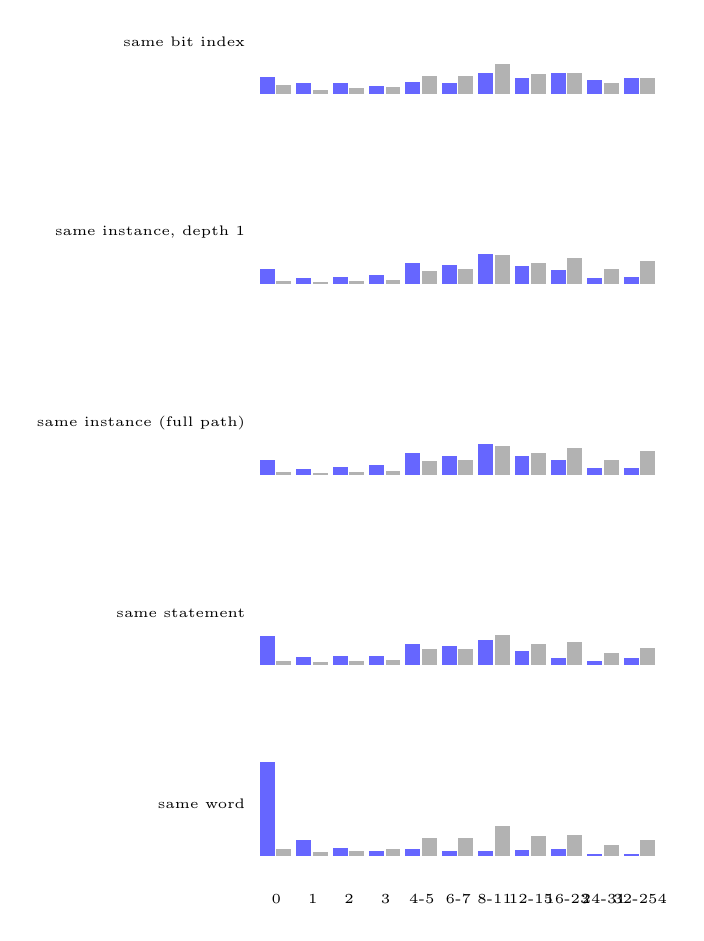
\begin{tikzpicture}[x=0.21cm,y=2.2cm,font=\tiny]
\node[anchor=east] at (-0.3,0.3) {same bit index};
\fill[blue!60] (0.0,0.0) rectangle (0.9,0.095);
\fill[gray!60] (1.0,0.0) rectangle (1.9,0.050);
\fill[blue!60] (2.2,0.0) rectangle (3.1,0.061);
\fill[gray!60] (3.2,0.0) rectangle (4.1,0.023);
\fill[blue!60] (4.4,0.0) rectangle (5.3,0.064);
\fill[gray!60] (5.4,0.0) rectangle (6.3,0.030);
\fill[blue!60] (6.6,0.0) rectangle (7.5,0.045);
\fill[gray!60] (7.6,0.0) rectangle (8.5,0.037);
\fill[blue!60] (8.8,0.0) rectangle (9.7,0.067);
\fill[gray!60] (9.8,0.0) rectangle (10.7,0.101);
\fill[blue!60] (11.0,0.0) rectangle (11.9,0.062);
\fill[gray!60] (12.0,0.0) rectangle (12.9,0.100);
\fill[blue!60] (13.2,0.0) rectangle (14.1,0.121);
\fill[gray!60] (14.2,0.0) rectangle (15.1,0.172);
\fill[blue!60] (15.4,0.0) rectangle (16.3,0.092);
\fill[gray!60] (16.4,0.0) rectangle (17.3,0.116);
\fill[blue!60] (17.6,0.0) rectangle (18.5,0.122);
\fill[gray!60] (18.6,0.0) rectangle (19.5,0.120);
\fill[blue!60] (19.8,0.0) rectangle (20.7,0.079);
\fill[gray!60] (20.8,0.0) rectangle (21.7,0.063);
\fill[blue!60] (22.0,0.0) rectangle (22.9,0.093);
\fill[gray!60] (23.0,0.0) rectangle (23.9,0.089);
\node[anchor=east] at (-0.3,-0.8) {same instance, depth 1};
\fill[blue!60] (0.0,-1.1) rectangle (0.9,-1.012);
\fill[gray!60] (1.0,-1.1) rectangle (1.9,-1.083);
\fill[blue!60] (2.2,-1.1) rectangle (3.1,-1.064);
\fill[gray!60] (3.2,-1.1) rectangle (4.1,-1.088);
\fill[blue!60] (4.4,-1.1) rectangle (5.3,-1.056);
\fill[gray!60] (5.4,-1.1) rectangle (6.3,-1.082);
\fill[blue!60] (6.6,-1.1) rectangle (7.5,-1.046);
\fill[gray!60] (7.6,-1.1) rectangle (8.5,-1.078);
\fill[blue!60] (8.8,-1.1) rectangle (9.7,-0.976);
\fill[gray!60] (9.8,-1.1) rectangle (10.7,-1.022);
\fill[blue!60] (11.0,-1.1) rectangle (11.9,-0.989);
\fill[gray!60] (12.0,-1.1) rectangle (12.9,-1.012);
\fill[blue!60] (13.2,-1.1) rectangle (14.1,-0.924);
\fill[gray!60] (14.2,-1.1) rectangle (15.1,-0.933);
\fill[blue!60] (15.4,-1.1) rectangle (16.3,-0.993);
\fill[gray!60] (16.4,-1.1) rectangle (17.3,-0.977);
\fill[blue!60] (17.6,-1.1) rectangle (18.5,-1.017);
\fill[gray!60] (18.6,-1.1) rectangle (19.5,-0.947);
\fill[blue!60] (19.8,-1.1) rectangle (20.7,-1.063);
\fill[gray!60] (20.8,-1.1) rectangle (21.7,-1.013);
\fill[blue!60] (22.0,-1.1) rectangle (22.9,-1.061);
\fill[gray!60] (23.0,-1.1) rectangle (23.9,-0.965);
\node[anchor=east] at (-0.3,-1.9000000000000001) {same instance (full path)};
\fill[blue!60] (0.0,-2.2) rectangle (0.9,-2.112);
\fill[gray!60] (1.0,-2.2) rectangle (1.9,-2.183);
\fill[blue!60] (2.2,-2.2) rectangle (3.1,-2.164);
\fill[gray!60] (3.2,-2.2) rectangle (4.1,-2.188);
\fill[blue!60] (4.4,-2.2) rectangle (5.3,-2.156);
\fill[gray!60] (5.4,-2.2) rectangle (6.3,-2.182);
\fill[blue!60] (6.6,-2.2) rectangle (7.5,-2.146);
\fill[gray!60] (7.6,-2.2) rectangle (8.5,-2.178);
\fill[blue!60] (8.8,-2.2) rectangle (9.7,-2.076);
\fill[gray!60] (9.8,-2.2) rectangle (10.7,-2.122);
\fill[blue!60] (11.0,-2.2) rectangle (11.9,-2.089);
\fill[gray!60] (12.0,-2.2) rectangle (12.9,-2.112);
\fill[blue!60] (13.2,-2.2) rectangle (14.1,-2.024);
\fill[gray!60] (14.2,-2.2) rectangle (15.1,-2.033);
\fill[blue!60] (15.4,-2.2) rectangle (16.3,-2.093);
\fill[gray!60] (16.4,-2.2) rectangle (17.3,-2.077);
\fill[blue!60] (17.6,-2.2) rectangle (18.5,-2.117);
\fill[gray!60] (18.6,-2.2) rectangle (19.5,-2.047);
\fill[blue!60] (19.8,-2.2) rectangle (20.7,-2.163);
\fill[gray!60] (20.8,-2.2) rectangle (21.7,-2.113);
\fill[blue!60] (22.0,-2.2) rectangle (22.9,-2.161);
\fill[gray!60] (23.0,-2.2) rectangle (23.9,-2.065);
\node[anchor=east] at (-0.3,-3.0000000000000004) {same statement};
\fill[blue!60] (0.0,-3.3000000000000003) rectangle (0.9,-3.129);
\fill[gray!60] (1.0,-3.3000000000000003) rectangle (1.9,-3.276);
\fill[blue!60] (2.2,-3.3000000000000003) rectangle (3.1,-3.253);
\fill[gray!60] (3.2,-3.3000000000000003) rectangle (4.1,-3.282);
\fill[blue!60] (4.4,-3.3000000000000003) rectangle (5.3,-3.246);
\fill[gray!60] (5.4,-3.3000000000000003) rectangle (6.3,-3.275);
\fill[blue!60] (6.6,-3.3000000000000003) rectangle (7.5,-3.244);
\fill[gray!60] (7.6,-3.3000000000000003) rectangle (8.5,-3.267);
\fill[blue!60] (8.8,-3.3000000000000003) rectangle (9.7,-3.179);
\fill[gray!60] (9.8,-3.3000000000000003) rectangle (10.7,-3.205);
\fill[blue!60] (11.0,-3.3000000000000003) rectangle (11.9,-3.191);
\fill[gray!60] (12.0,-3.3000000000000003) rectangle (12.9,-3.203);
\fill[blue!60] (13.2,-3.3000000000000003) rectangle (14.1,-3.151);
\fill[gray!60] (14.2,-3.3000000000000003) rectangle (15.1,-3.124);
\fill[blue!60] (15.4,-3.3000000000000003) rectangle (16.3,-3.219);
\fill[gray!60] (16.4,-3.3000000000000003) rectangle (17.3,-3.177);
\fill[blue!60] (17.6,-3.3000000000000003) rectangle (18.5,-3.256);
\fill[gray!60] (18.6,-3.3000000000000003) rectangle (19.5,-3.163);
\fill[blue!60] (19.8,-3.3000000000000003) rectangle (20.7,-3.274);
\fill[gray!60] (20.8,-3.3000000000000003) rectangle (21.7,-3.228);
\fill[blue!60] (22.0,-3.3000000000000003) rectangle (22.9,-3.257);
\fill[gray!60] (23.0,-3.3000000000000003) rectangle (23.9,-3.201);
\node[anchor=east] at (-0.3,-4.1000000000000005) {same word};
\fill[blue!60] (0.0,-4.4) rectangle (0.9,-3.856);
\fill[gray!60] (1.0,-4.4) rectangle (1.9,-4.362);
\fill[blue!60] (2.2,-4.4) rectangle (3.1,-4.311);
\fill[gray!60] (3.2,-4.4) rectangle (4.1,-4.378);
\fill[blue!60] (4.4,-4.4) rectangle (5.3,-4.354);
\fill[gray!60] (5.4,-4.4) rectangle (6.3,-4.370);
\fill[blue!60] (6.6,-4.4) rectangle (7.5,-4.370);
\fill[gray!60] (7.6,-4.4) rectangle (8.5,-4.362);
\fill[blue!60] (8.8,-4.4) rectangle (9.7,-4.361);
\fill[gray!60] (9.8,-4.4) rectangle (10.7,-4.298);
\fill[blue!60] (11.0,-4.4) rectangle (11.9,-4.373);
\fill[gray!60] (12.0,-4.4) rectangle (12.9,-4.299);
\fill[blue!60] (13.2,-4.4) rectangle (14.1,-4.371);
\fill[gray!60] (14.2,-4.4) rectangle (15.1,-4.225);
\fill[blue!60] (15.4,-4.4) rectangle (16.3,-4.367);
\fill[gray!60] (16.4,-4.4) rectangle (17.3,-4.283);
\fill[blue!60] (17.6,-4.4) rectangle (18.5,-4.359);
\fill[gray!60] (18.6,-4.4) rectangle (19.5,-4.278);
\fill[blue!60] (19.8,-4.4) rectangle (20.7,-4.389);
\fill[gray!60] (20.8,-4.4) rectangle (21.7,-4.335);
\fill[blue!60] (22.0,-4.4) rectangle (22.9,-4.390);
\fill[gray!60] (23.0,-4.4) rectangle (23.9,-4.309);
\node at (1.0,-4.6499999999999995) {0};
\node at (3.2,-4.6499999999999995) {1};
\node at (5.4,-4.6499999999999995) {2};
\node at (7.6,-4.6499999999999995) {3};
\node at (9.8,-4.6499999999999995) {4-5};
\node at (12.0,-4.6499999999999995) {6-7};
\node at (14.2,-4.6499999999999995) {8-11};
\node at (16.4,-4.6499999999999995) {12-15};
\node at (18.6,-4.6499999999999995) {16-23};
\node at (20.8,-4.6499999999999995) {24-31};
\node at (23.0,-4.6499999999999995) {32-254};
\end{tikzpicture}
\caption{Round 7 (exploratory): distribution of the placed Manhattan distance (CLB units, mean over ten stock seeds) of pairs with the HDL relation (blue) and without it (gray), per relation, pooled over designs; bars are shares of each group.}
\label{fig:r7dist}
\end{figure}
